

\section{An Alternative Vision Framework}
Current pattern recongition systems are far from the capabilities of the biological system.
For example, when a human looks at a dog, his brain can immediately construct a model of it, 
including body schema, motion pattern, shape and attitude of body and limbs and texture of its surface.  
This internal representation is seamlessly integrated with the emotional and the motor-planning system, so that we can touch and behaviorally interact with it.

My, and presumably my supervisors', long-term vision is the implementation of such a system. In order to solidify this vision, a number of inquiries need to be answered: What kind of data structure is used to express the representation of the dog? How does this representation emerge through interaction with sensory signals? And how is the whole structure created and acquired through learning? It seems obvious that the representation of the cat is built from pre-existing or already learned partial descriptions (``net fragments'') that have a certain degree of adaptability and can only be combined in certain ways.
Based on our understanding of the brain, the current representation of the dog and how it connects with the sensory system, motor system, and behavioral control system can be described as a large group of active neurons and their connections. This network is embedded in a continuum of neighboring networks.

One of the insights from the \emph{Gestalt} psychology is that humans are apparently able to recognize the Gestalt of an object within a very short time; The brain can immediately recognize global patterns - arrays of local features that consistently conform to a known large-scale pattern - even if those local features are buried in noise or would, on the basis of local context, be interpreted very differently. Thus, local decisions should be made based on plausibility considering overall patterns, while the overall patterns can only be defined based on local features.

Therefore, for the extraction of features from images, it is important to avoid the ``fallacy of early commitment'' as David Marr put it \sidecite{Marr_2010}. In contrast, this ability is not apparent in current neural network. Although some of the progress yields results that might give the illusion of this capability, knowledge about the underlying mechanics suggest that neural networks do not possess the same ability at Gestalt recognition as we do: The first layers of deep networks, which extract features from images, typically consider only local patches whose features are compress in later layers. Thus, the first layer do not consider global features but steer the decision process towards specific classes. Therefore, deep network take local decisions without consolidating global information.

Some essential aspects of this vision can be realised in a simple model of invariant object recognition composed of two layers, L1 and L2 and a system of projection fibers that run between L1 and L2 (L1 could stand for primary visual cortex, and L2 for an area in temporal cortex).
In this context, layer refers not to a layer of an artificial network but to a network consisting of a multitude of neuronal layers.
The first layer L1 serves as feature extractor, while the second layer L2 represents object representations. The projection fibers map, in an iterative process, the features from L1 to the object representations in L2 and vice versa.

In this thesis, a first step towards the implementation of this vision is taken. Thereby, the main focus is on the implementation of the feature extractor (L1).
TODO Text.

\subsection{Feature Extraction (L1)}
The humans mechanism implementing the Gestalt phenomenon allows to recognize the Gestalt of an object within a very short time. The ability of this mechanism is rooted in lateral connections, which are recurrent connections operating at the same level of features. Unlike feed-forward connections that ascend through a hierarchy of feature detectors, these lateral connections enable elementary feature neurons to be activated by input and briefly fire. However, their continued firing relies on receiving support from a sufficient number of other activated neurons, which are also connected to them. Initially activated neurons that do not receive enough lateral support deactivate after a short period. Consequently, a significant response involves a collective group of neurons that mutually support each other through connections. Therefore, it is essential to view the process from the perspective that the winning neurons are integral parts of consistent networks of connections, enabling them to persist beyond the transient phase. These consistent networks are the high-level patterns discussed in the Gestalt movement. Hence, the aforementioned  conundrum, that local decisions should be taken on the basis of plausibility in the light of high-level patterns while the high-level patterns can only be defined on the basis of low-level features, is resolved by the fact that the input activates numerous feature neurons that fit the local input, but the high-level patterns represented by coherent networks of lateral connections only select those that are mutually consistent in terms of the overall pattern.

The connections present in L1 possess the capacity to represent an extensive array of consistent connectivity patterns. Each neuron within L1 exhibits multiple excitatory incoming and outgoing connections, allowing it to be involved in slight variations and deformations of a specific pattern, as well as completely distinct global patterns. However, due to the limited range of lateral connections, coherence is maintained only within that particular range. In order to represent larger-scale structures like that of a dog, longer-range connections become essential, and these are found in L2. In L2, patterns remain invariant to translation, scale, and orientation, enabling the incorporation of broader spatial relationships.

\subsection{Object Representations (L2)}
Layer L2 exhibits a structure similar to L1, with a few distinctions. It has a smaller coverage area, focusing specifically on object-centered representations rather than encompassing the entire visual field. Additionally, L2 enables connections with an extended range, spanning a significant portion of the object's representation.

In the object recognition process, a comprehensive network plays a central role: It consists of a sub-network within L1 that covers the region of the visual field containing the object, as well as a sub-network in L2 that represents the object. Active projection fibers, or axons, connect corresponding neurons in the L1 and L2 networks. Here, ``corresponding'' refers to neurons relating to the same point on the object's surface.

The fiber projection between the L1 and L2 networks is composed of ``maplets''. A maplet comprises a collection of fibers that establish one-to-one connections between all neurons in a small patch of L1 and all neurons in a small patch of L2 in a topological manner. This topological connection links neighboring neurons in L1 to neighboring neurons in L2. Both L1 and L2 are divided into overlapping patches, and for each pair of patches—one in L1 and one in L2—a corresponding maplet exists.

When the proper control units observe a high pattern correlation between the fibers reaching L2 and the local neural activation pattern there, they initiate activation. They inhibit competing units and stabilize the network in L2 using the activated fibers. Consequently, the activated projection achieves a homeomorphism, where neurons of a particular feature type in L1 are connected to neurons of the same type in L2. Furthermore, neighboring neurons in L1 project to connected neurons in L2.



\section{Probabilistic Framework}
The previous section presented an alternative vision framework, that implements the Gestalt phenomena by design. It is based on local subnetworks that emerge over short amounts of time. Subnetworks comprise neurons supporting each other to remain active.
When presented with the same input, t an attractor state will be reached. This implies the formation of a stable subnetwork of neurons that persists as long as the input remains unchanged or undergoes minimal alterations. Consequently, neurons within this network mutually reinforce one another, utilizing fundamental principles to provide support:

\begin{itemize}
    \item When a relatively small amount of synapses are active (10 out of 10'000 connections), the neuron is active. 
    \item Activation is sparse. That is, at each point in time only a fraction of neurons is active.
    \item Neurons that tend to fire simultaneously tend to form stronger bonds (Hebbian update rule).
    \item The connections are lateral and not feedforward only. This implies a time-dependency used to form the subnetworks. 
\end{itemize}

These characteristics differ from typical feed-forward architectures in several ways.  In traditional neural networks, neurons exhibit dense activity, meaning that even with the application of the Rectified Linear Unit (ReLU) activation function, approximately 50\% of neurons remain active (above zero). Consequently, all synapses are active, and a neuron is represented as the weighted sum of all neurons from the previous layer, without incorporating lateral connections. Furthermore, temporal dynamics are absent, as neural networks are typically perceived as functions that promptly process an input and generate an output. Therefore, one can conceptualize a neural network as $\boldsymbol{y} = f(\boldsymbol{x})$. Even autoregressive models adhere to this structure, where $\boldsymbol{y}_t = f(\boldsymbol{y}_{t-1})$.

This suggests that implementing subnetworks requires using different principles than the ones used in classical neural networks. Therefore, a probabilistic framework based on probabilistic neurons is introduced.
A probabilistic neuron is a binary neuron that does not fire when a certain threshold is reached but uses its internal state as firing probability.

This is a different principle than neural networks that deal with probabilities, such as probabilistic neural networks (PNN) \sidecite{Mohebali_Tahmassebi_Meyer_Baese_Gandomi_2020}. PNNs were already introduced in 1967 by D.F. Specht \cite{Specht_1967, Specht_1990} and are well suited for classification and allocate the class with highest posterior probability to new input data \cite{Zeinali_Story_2017}.
In contrast to PNNs, the proposed framework is based on \emph{probabilistic neurons} and does not model class but activation probabilities.

A probabilistic neuron $x_i$ is modelled as a probability density function of the form:
\begin{equation}
    p(x_i = \text{active} | \text{activity of neighborhood}, \text{environment}) 
\end{equation}

Thus, the probability of neuron being active depends on the activity pattern of the neurons in its local neighborhood and factors of the environment (e.g., inhibition or presence of neurotransmitters).
Such a neuron can be implemented using a Bernoulli distribution, i.e., $B(p) = P(X = 1) = p = 1 - P(X=0)$. Having a neuron whose firing probability $p$ is governed by the activity of the neighborhood and the environment allows to implemented the behaviour of subnetworks: After receiving an input, the neurons get excited and fire with a higher probability. However, their fire probability decreases quickly if not supported by neighboring neurons. Thus, uncertainty and potential subnets govern timestep 0 while shortly after the network reaches an attractor state. In the following, some advantages of probabilistic neurons are pointed out before a concrete implementation of subnetworks is proposed.


\begin{figure}[h]
    \centering
    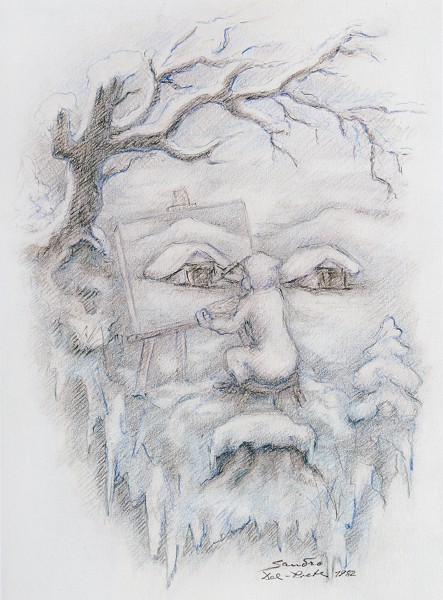
\includegraphics[width=0.99\textwidth]{sdp_mountain_spirit.jpg}
    \caption[Mountain Spirit in Winter by Sandro del Prete]{Mountain Spirit in Winter by Sandro del Prete. The image is from \citeay{sdp_mountain}.}
    \figlbl{sdp_mountain}
\end{figure}


\paragraph{Ambiguity.} Probabilistic neurons permit the persistence of multiple subnetworks, enabling the system to handle ambiguity effectively. For example, when presented with a composite face comprised of distinct objects (c.f. \figref{sdp_mountain}), both the subnetwork responsible for abstract faces and the subnetworks associated with individual objects become active concurrently. Consequently, one can attend to these subnetworks simultaneously, utilizing attention in its original sense rather than the conventional deep neural network (DNN) interpretation. I speculate that this represents a fundamental distinction from neural networks that are compelled to represent the entire scene within a single high-dimensional dense vector.

\paragraph{Interpretability.} The probabilistic frame allows for much better interpretability than classical deep networks. Each neuron can be part of a multitude of subnetworks and thus some semantic, i.e. corresponds to something meaningful. Furthermore, its internal state is a probability that can be interpreted as the networks confidence that this specific feature was observed in the input. A network of probabilistic neurons that support each other over timesteps can also be interpreted as a directed graph. This allows to trace how subnetworks are activated. Without formal proof or presenting an interpretability framework, I speculate that using this probabilistic framework will significantly simplify the explainability of intelligent systems.

\paragraph{Robustness.} A neural networks is usually represented with a vector which is sequentially processed by a mathematical functions (e.g. with neural layers). Artificial networks in particular are not robust to noise and are susceptible to adversarial attacks \sidecite{Akhtar_Mian_2018}. Slight changes to the input or a network-internal vector can completely falsify the overall result. This is because typical artificial networks work with continuous numbers and these feature vectors can consequently lie anywhere in the feature space. Therefore, a minimal change, e.g. triggered by noise, can shift the feature to the other side of the decision boundary and change the result. A binary vector, on the other hand, has different mathematical properties and is more robust against noise and adversarial attacks, especially if they are sparse and distributed\sidenote{only a small portion of the bits are ``on'', and representations differ by multiple binary bits} \sidecite{Ahmad_Hawkins_2015}.
Subsampled or noisy vectors are still semantically similar and are close to the original vectors when compared, for example by counting the overlap of bits between two vectors.

\section{Implementation}
TODO Add Overview of entire system


\subsection{Processing Loops}
\begin{figure}[h]
    \centering
    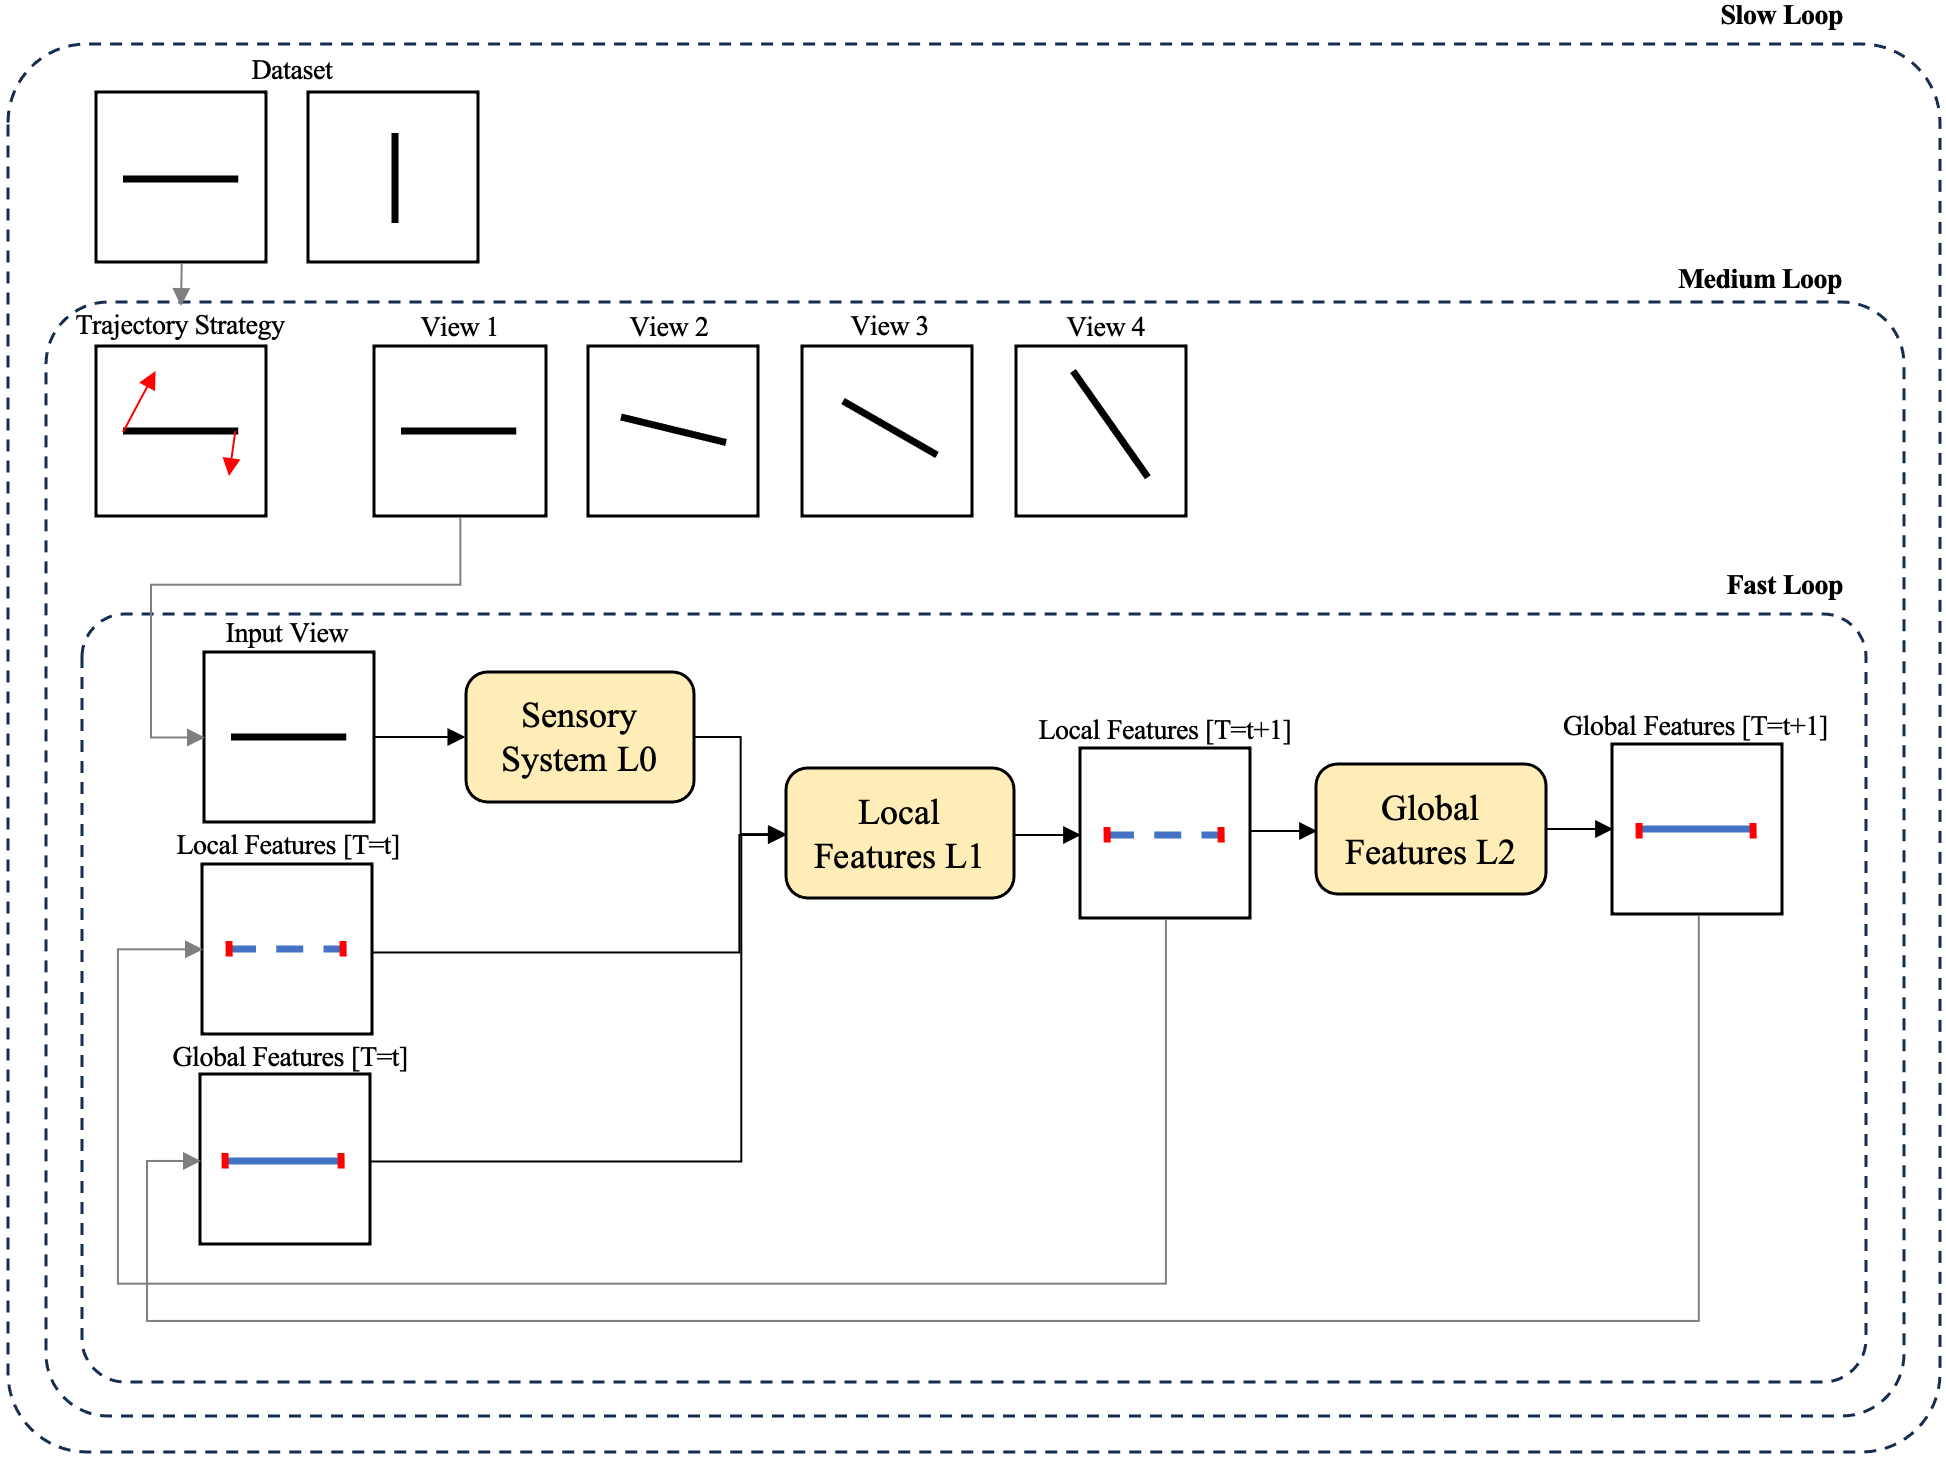
\includegraphics[width=0.99\textwidth]{lateral_loops.png}
    \caption[Processing loops of the network]{Processing loops of the network. From each sample in the dataset (slow loop), multiple views are generated (medium loop), and each view is processed over multiple timesteps by the model (fast loop).}
    \figlbl{lateral_loops}
\end{figure}
The proposed framework introduces nested learning cycles, each with a different functionality. Since the proposed framework runs on a tacked computer hardware, the cycles are bound to fixed timesteps. At each timestep, the innermost loops executes a step. As soon as the innermost loop is finished, an outer loops takes a step and the process is repeated.

\begin{itemize}
\item[\textbf{Slow Loop}] The dataset comprises $D$ images, with each image depicting a randomly generated line. The images are processed one after the other, building the outermost loop.
\item[\textbf{Medium Loop}] For each image in $D$, $V$ different views are sampled by slightly changing the image based on a trajectory strategy. This generates $V$ distinct yet visually similar images. Similar to our visual system, which captures multiple frames of an object before moving on to the next, this loop allows to perceive objects from various viewpoints.
\item[\textbf{Fast Loop}] From each view $V$, a sensory system creates neural activity that is processed by the network for $T$ timesteps. This loop allows the network to build subnetworks over several timesteps. First, the network has a high neural activity, which is quickly reduced within these $T$ steps as only the activations with enough lateral support remain active and convergence to an attractor state. At each timestep, the input (static) input from the sensory system as well as the previous cell state is fed into the network. The input of the sensory system is fed into the network to make it more stable. Intuitively, this can be compared to closing our eyes: When closing our eyes, we tend to forget the exact location of objects and thus our internal representation slightly shift away.
\end{itemize}


\subsection{Sensory Input}
An intelligent agent may have a multitude of sensory input. The main difficultly is that sensory input (especially images) are in continuous space, and they must be translated into an activation potential.
Thus, the sensory input must be linked to probabilistic neurons. Such a sensory system can be implemented by using either Gabor filters \sidecite{Gabor_1946, Granlund_1978} or, in a more advanced setting, with learned filters.
Such filters can be learned, for example, by training a deep network in a autoencoding setting \sidecite{rumelhart1985learning}. Even though such networks violate the principles from the Gestalt phenomena, their first layer exhibit excellent capabilities in extracting relevant features from images. Therefore, I argue that such filters are well suited as a network's sensory system if only the first layers are kept. However, also the output $\boldsymbol{h}$ of such as layer is not binary.
One option is to consider the normalized values of $\boldsymbol{h}$ as probabilities, with the notion that higher values indicate regions where a filter discovers matching features in the image. Alternatively, another approach involves setting all values in $\boldsymbol{h}$ above a pre-defined threshold to 1 and assigning 0 to the remaining values.
As a third option, quantization networks such as VQ-VAEs \sidecite{NIPS2017_7a98af17} can be used to map local features to a discrete value that can be translated in a binary activation pattern.

This thesis focuses on implementing a proof-of-concepts for handling straightforward images, which allows the utilization of a pre-defined hand-crafted sensory system. However, when processing complex natural images in future research, it is imperative to conduct empirical investigations to explore these possibilities further.

\subsection{Feature Extractor (L1)}
\begin{figure}[h]
    \centering
    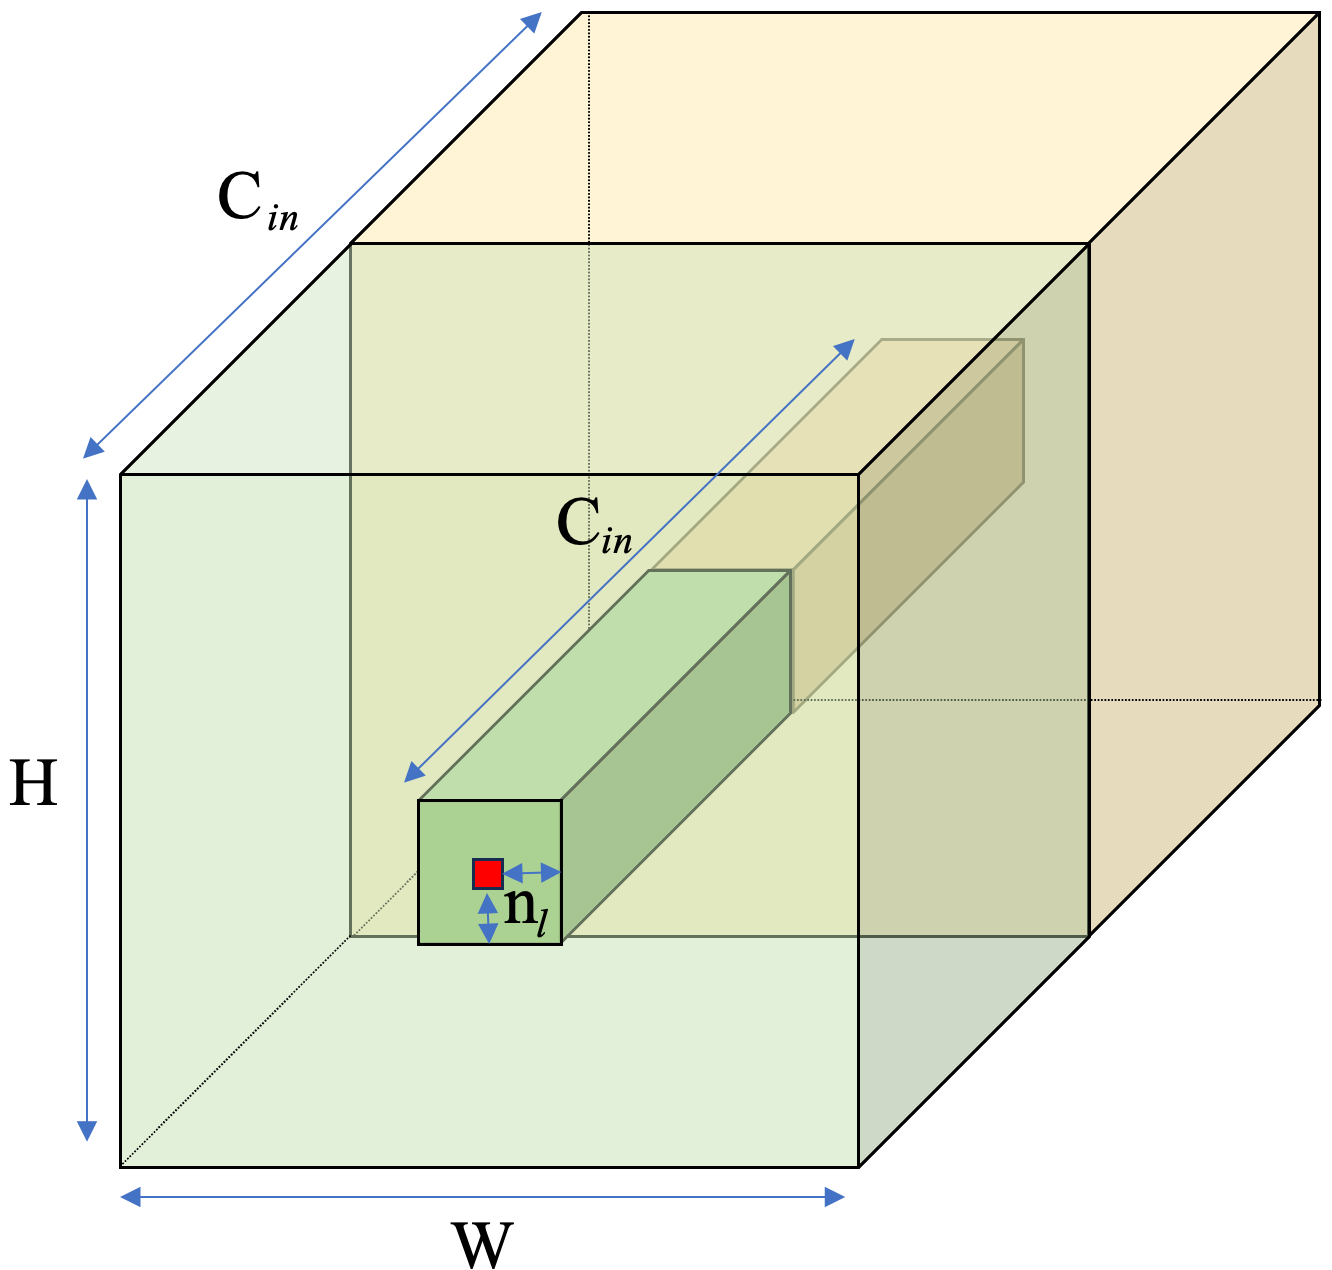
\includegraphics[width=0.99\textwidth]{local_neighbourhood.png}
    \caption[Laterally connected cells]{Visualization of the laterally connected cells: The red cell of an array of cells of the size $C \times W \times H$ is laterally connected to an neighbourhood of size  $C \times 2n \times 2n - 1$ ($-1$ representing the red cell itself).}
    \figlbl{local_neighbourhood}
\end{figure}
The sensory system converts an image into a binary observation of size $C_{in} \times W \times H$ where $C_{in}$ is the number of input channels, $W$ the image width and $H$ the image height.
Our network implements one cell for each binary observation, leading to $C_{in} \times W \times H$ cells.
Having multiple input channels means having multiple cells at the same pixel location, representing one of $C_{in}$ feature.

Let's denote a cell of feature channel $c \in \{0, ..., C_{in}\}$ at position $w \in \{0, ..., W\}$, $h \in \{0, ..., H\}$ as $x_{c,w,h}$.
Each cell's activation is supported by neighbouring cells through lateral connections. Let's define the reach of lateral connections along the vertical and horizontal axis of an image as $n$.
Furthermore, the cells are also laterally connected across the channels, allowing a cell be supported from other cells representing different features.
Therefore, each cell has $C\cdot n^2 - 1$ laterally connected cells at the positions $\{x_{0,w-n,h-n}, ..., x_{C,w+n,h+n}\} \\ x_{c,w,h}$. This lateral connectivity is also depicted in \figref{local_neighbourhood}. 

A known pattern should excite the cells and the cells should remain active through lateral support. 
However, the pattern can appear at any position within the image, requiring the lateral support to be position equivariant.
Computer vision architectures solve this problem with convolutional filters shifting over each pixel location. This mechanism can also be used for implementing the lateral connections: When using a convolutional kernel with size $C_{in} \times 2n+1 \times 2n+1$, the state of a cell is updated based on the local neighbourhood. This local neighbourhood are the laterally connected cells and the learned weights of the kernel is the weight of their support.
Thus, lateral support is implemented as


\begin{align}\eqlbl{convlat_1}
	\Delta w_{ij} = \eta x_i x_j
\end{align}


\subsubsection{Hebbian Updates}
The human brain's learning algorithm is based on local self-orgnisation and unsupervised (or self-supervised) learning \sideciteay{von_der_Malsburg_Stadelmann_Grewe_2022}. The biologically most plausible learning algorithm is Hebbian learning \sidecite{Hebb_1949}. Hebbian learning can be summarized as ``neurons that fire together wire together'' (c.f. \secref{Hebbian}).
This learning rule is well suited for learning lateral connections: If two cells are active together (``fire together''), their weight is increased (``wire together''). During training, the cells are activated is a specific pattern based on the sensory input. Hebbian learning strengthens the connections between the cells that are active at the same time, i.e. increasing the lateral support between these cells. Furthermore, the weight (i.e. the strength of the lateral support) is reduced between between cells that fire in disparity (one of the cells is firing while the other is not).
Thus, Hebbian learning is the algorithm to learn lateral support while being biologically plausible.

The weight $w_{ij}$ between two binary cells $x_i$ and $x_j$ is increased, when they are active at the same time. The weight update $\Delta$ can be calculated as follows, leading to an increase of $w_{ij}$ by $\eta$.

\begin{align}\eqlbl{hebbu_1}
	\Delta w_{ij} = \eta x_i x_j
\end{align}

The formula above leads to an increase when both neurons are active at the same time. To decrease lateral support between cells where only one cell is active, the formula can be extended as follows:

\begin{align}\eqlbl{hebbu_2}
	\Delta w_{ij} = \eta \left( x_i x_j + (x_i-1) x_j + x_i (x_j -1) \right)
\end{align}

The term $(x_i-1) x_j$ becomes $-1$ if the $x_i=0$ and $x_j=1$ and thus decreases the weight if these cells are firing disparity. The second term $x_i (x_j -1)$ implements the same behaviour for the other cell ($x_i=1$ and $x_j=0$).

So far, only the update between two cells is discussed. However, the network consists of multiple cells whose lateral connection strength is defined by a kernel $\boldsymbol{W}$. This kernel has the size $C_{out} \times C_{in} \times 2n+1 \times 2n+1$. Thus, the activity of a cell is calculated based on different weights connecting all neighbouring cells.

During training, the network might see similar patterns multiple times, leading to very strong connections between specific cells. In order that these lateral connection strengths cannot grow to infinite, the weight is normalized. The weights are normalized per output channel, ensuring that the post-synaptic activity cannot get too high. 

\begin{align}\eqlbl{hebbu_2}
	\boldsymbol{W(C_{out})} = \boldsymbol{W(C_{out})} / (1\cdot 10^{-10} + \sqrt{\sum_{ci}^{C_{in}}\sum_{w}^{2n+1}\sum_{h}^{2n+1} \boldsymbol{W(C_{out},ci,w,h)}})
\end{align}


\paragraph{Breaking the Symmetry.}  Oja \cite{Oja_1982} showed that the Hebbian learning rule converges for linear neurons to the first principle component of the input data. He concluded that a 
network of such neurons appears not very useful, as all neurons will just learn the first principle component and that an additional element is required providing differentiation between the neurons.
In practice, this additional element is typically some kind of competition such as winner-take-all. With winner-take-all, only the neuron with the highest activation is selected for learning. In the case of of our network with lateral connections, this means that at each pixel location exactly one of the feature channels $C$ is updated. However, this not desirable: Imagine a pixel region with no activation: In this area, we don't want to learn any support between neurons as there is no activity. However, with winner-take-all, we enforce one channel to be active and thus learn lateral support between this enforced activity. However, we found that no measures are necessary at all. The probabilistic neuron is able to break the symmetry. When using the probabilistic neuron, neurons are activated with e certain probability. This probability provides enough differentiation between cells, 
making a competition strategy superfluous.

\paragraph{Implementation Details.} Implementing Hebbian updates efficiently in a deep learning framework is not trivial: In an efficient implementation, the kernel is not shifted from cell to cell but a circulant matrix is built so that all kernel updates can be calculated in parallel. However, by applying this operation, information about the cell's lateral influence is lost. One way to efficiently implement Hebbian learning for convolutional operations is to use special loss functions. Miconi \cite{Miconi_2021} proposes to use a loss function whose derivative is exactly the Hebbian update. By doing so, backpropagation of error can be used to update the weights. In this thesis, a different implementation is used that comes with a slight memory overhead but is very efficient and does not rely on backpropagation at all. Furthermore, it gives much more flexibility and allows to implemented different normalization strategies. Instead of using a forward pass through a convolutional layer with subsequent backward pass, my implementation uses two convolutional layers without backward pass. The first layer is a fixed, binary convolution that restructures each input patch into a single column vector. This is followed by a $1\times1$ convolution containing the actual weights. Specifically, we can pass the input through a fixed convolution with an input size of $C_{in} \times 2n+1 \times 2n+1$ and $C_{in} 2(2n+1)$ output channels. The weight vector for this convolution is set to $1$ for the connections linking input $c_i,w,h$ to output $c_iwh$ (where $c_i$ $w$, and $h$ range from 1 to $C_{in}$, $2n+1$, and $2n+1$, respectively), and it is set to 0 everywhere else. This process reorganizes the values of each input patch from the original convolution into non-overlapping column vectors, effectively duplicating them. Next, we can apply the actual weights of the original convolution using a simple $1\times1$ convolution. This can be achieved by performing a tensor product with appropriate broadcasting.


\subsubsection{Initialization}\seclbl{lateral_init}
\begin{figure}[h]
    \centering
    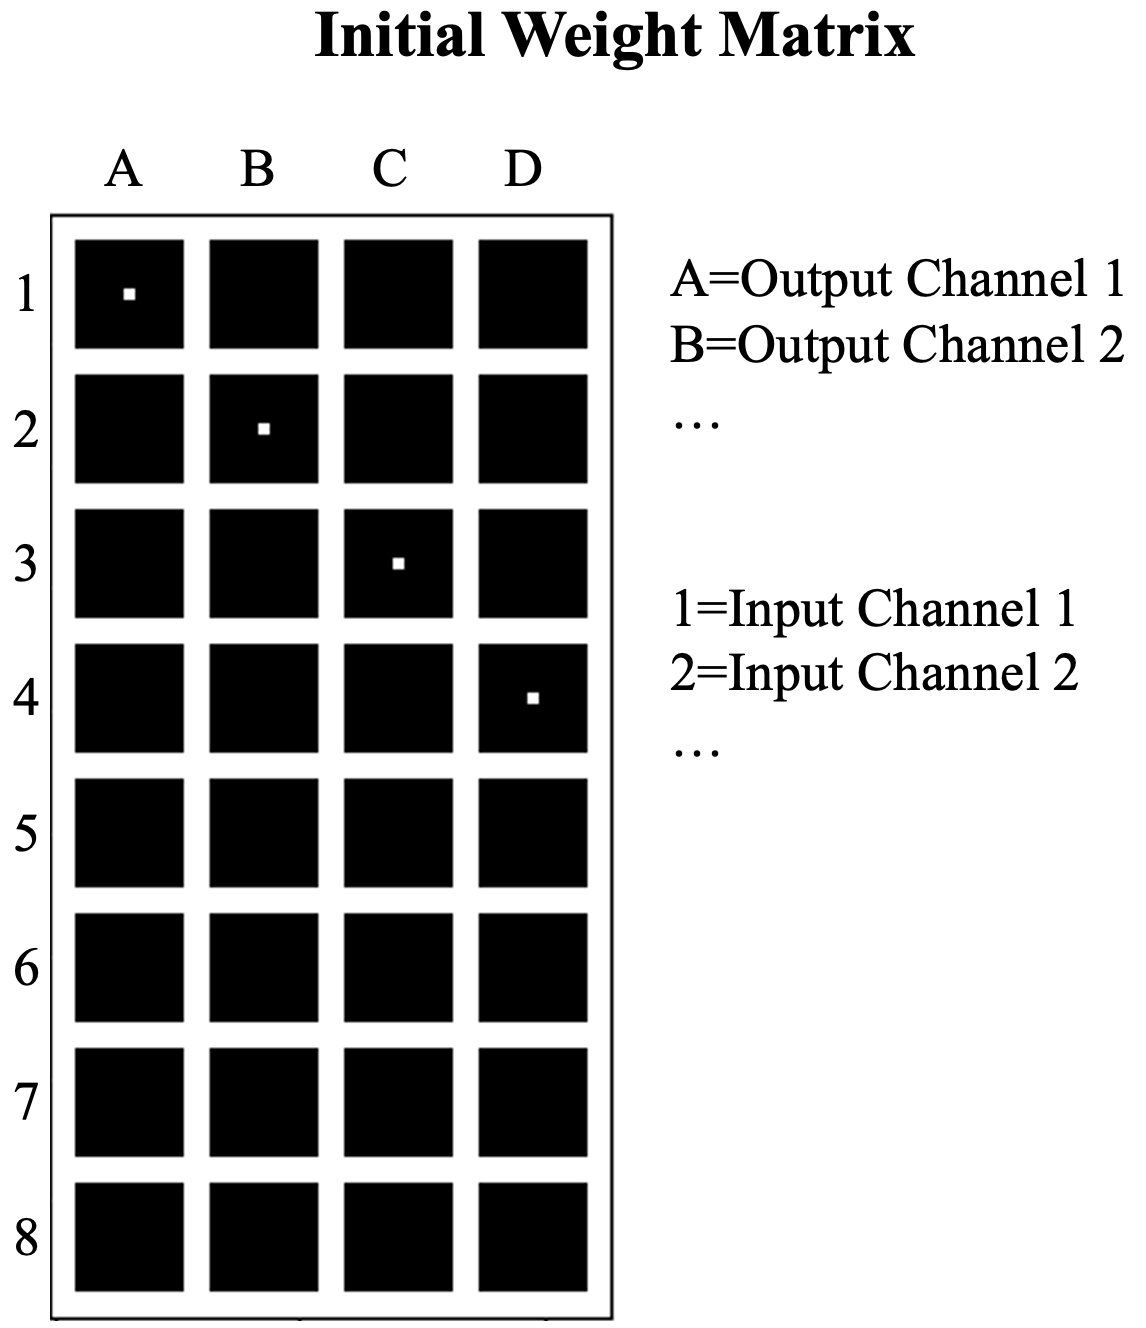
\includegraphics[width=0.99\textwidth]{lateral_init_weights.png}
    \caption[Initialization of the lateral weight matrix]{Initialization of the lateral weight matrix. The weight at the middle of a kernel, whose input and output channel have the same index, is set to $1$.}
    \figlbl{lateral_init_weights}
\end{figure}
The lateral support is implemented as weights of a convolutional kernels.
It is crucial to initialize these kernels properly, otherwise, the activations are not stable and typically converge to weights that either activate all cells or none cells.
For example, when the kernels are initialized with zeros, there is no lateral support and all cells will turn off immediately.
If the weights are initialized randomly, the initial support is random and patterns that are not in the training set  are supported.

I found that it works best if the weights are initialized with a high self-support, meaning each cell supports itself to remain active.
Self-support can be implemented by setting all weights of a kernel of size $C_{out} \times C_{in} \times w \times h$ to $1$ at the indexes that fulfil 
$C_{out} = C_{in}$, $w = n+1$, and $h = n+1$. Thus, the weight at the middle of a kernel that has the same input as output channel is set to $1$ while the other weights are set to $0$. This initialization strategy also works for kernels with a different number of input and output channels as shown in \figref{lateral_init_weights}.

Having such a weight matrix ensures that the cells activation at time $t$ and at time $t+1$ is exactly identical. However, after applying the Hebbian learning rule, the weights are updated in a way to capture the data's statistics.


\subsubsection{Normalization}
The lateral support defines the probability of a neuron to be active. However, the output of a convolutional operation is not in the range $0, ..., 1$ but can be any floating point number. Thus, this numbers have to be normalized to represent a probability.
Normalizing is quite challenging for the following reasons:
\begin{itemize}
	\item The lateral support increases over time: The lateral weights are initialized by only having self-support. However, the network's cells learn to support each other based on the data's statistics. This has the effect, that neurons become stronger activations during the course of the training process. For example, a single cell can have a binary value of $1$ at the beginning. This cell supports itself, i.e. keeps the $1$ at the beginning. After Hebbian updates, this self-support can either go towards $0$ and the cells turn off or can be supported by up to $n^2$ cells. The support strength of each of these cells can be in the range $-1, ..., 1$. Thus, a cell can have an activation up to $n^2+1$. The challenge hereby is that its initial support is $1$ and then evolves to a complete different value even if the data remains identical. Thus, the support needed to remain active must be low at the beginning of the training and be slowly increased during training until an upper bound is reached.
	\item The possible support depends on the input data: The sensory system extracts different features from the input data. Depending on the input data, there can be regions with a lot of detected features and regions with less features. For example, some areas can be constituted from many edges, and well pronounced structures leading to a lot of activations in various channels (e.g. a zebra within an image) while other areas have rather low frequencies and only a few activations (e.g. the sky in the background of the zebra image). However, even though areas have only a few activations, they should not just be turned off. Otherwise, the network would only keep features of areas with a high frequency and discard all other information.
\end{itemize}

Thus, the support depends on the learned lateral weights that change slowly during training and the input data that change every time a new scene is observed.
The problem with the changing weights can be solved by dividing the cells' activation by the sum of the lateral weights.
This normalization is done per feature channel. This allows to deal with the problem that different features receive a different strong support.
By doing so, more lateral support is needed to remain active when more lateral connections are learned: At the beginning, only self-support exists and thus the sum of the weight is $1$. Therefore, a cells activation is divided by $1$ and being active at time $t$ is enough to be active at time $t+1$.
However, during training, more lateral connections are build (i.e. more weights become $>1$). Therefore, a cells activation is divided by a value $>1$ and the activation has to be stronger to remain active with a high probability.
Mathematically, the normalization of an array of cells with an activation strength $\boldsymbol{A}(out)$ per feature channel is defined as follows:
\begin{align}\eqlbl{norm_lat}
	\boldsymbol{A}(out) :=  \boldsymbol{A}(out) / (1\cdot 10^{-10} + \sum_{ci}^{C_{in}}\sum_{w}^{2n+1}\sum_{h}^{2n+1} \boldsymbol{W(C_{out},ci,w,h)})
\end{align}

The problem that has to be solved is that the sensory system detect different features in different image areas and thus that an image's feature map depends highly on the input data. Therefore, the activations have to be normalized depending on the input data. This problem is solved by counting haw many cells are active in the lateral neighbourhood, i.e. by counting how many cells that potentially could support a cell are active.
This can be implemented efficiently by applying a convolutional operation on the input, whereby the kernel has a size of $C_{out} \times C_{in} \times 2n+1 \times 2n+1$ and all weights are set to $1$. The result of this operation is a matrix $A_{max}$, describing for each cell what its maximum activation could be for a given input.
The activations are divided element-wise by $\boldsymbol{A}_{max}$ so that they are normalized based on the sensory system's activation pattern.
\begin{align}\eqlbl{norm_lat2}
	\boldsymbol{A}(C,w,h) :=  \boldsymbol{A}(C,w,h) / \boldsymbol{A}_{max}(C,w,h)
\end{align}

The above described operations normalize the activations in a sense that they are independent from the strength of the lateral connections as well as from the input data. However, they are not bound to the range $0, ..., 1$ and, thus, not usable as probabilities.
To squeeze the activations values inside these range, min-max normalization is used.  

\begin{align}\eqlbl{norm_lat3}
	\boldsymbol{A}(C,w,h) :=  \boldsymbol{A}(C,w,h)  - \min(\boldsymbol{A}) / (\max(\boldsymbol{A}) - \min(\boldsymbol{A}))
\end{align}


\subsubsection{Measuring Support Goodness}
An open challenge from this approach is to define how good a trained network works.
A simple approach is to measure the support needed to remain active.
A simple metric is to measure the average support active and inactive cells receive.
At the beginning of training, self-support is used, i.e. it is sufficient to be active at time $t$ to remain active at $t+1$.
Therefore, the average support of active cell is $1$ and the average support of inactive cells is $0$.
However, during training, lateral connections are learned that support cells to remain active.
This leads to a higher activation in general which, in turn, increases the threshold to remain active.
Thus, the average activation of the cell increases as well as the threshold to remain active.
In a working system, the activation needed to become active increases during training.
We measure this statistics to evaluate the goodness of the subnetworks.

As a second metric, I measure the normalization factor.
The cells are activation with a specific strength based on the input and the lateral support they receive.
However, the normalization squeezes this activation into the range $0, ..., 1$.
If the cells are activated with a specific activation strength $A$ and normalized afterwards to $A_{norm}$, we can measure the normalization factor 
$\upsilon$:
\begin{align}\eqlbl{goodness_lat}
	\upsilon = \frac{A}{A_{norm}+1\cdot10^{-10}}
\end{align}
At the beginning, the cells do not receive a lot of support and thus $\upsilon$ is small. However, with increasing support, $\upsilon$ increases and indicates that a higher activation strength is needed to become active.

As a third goodness measurement, we can measure the robustness to noise.
The subnetworks consists of cells supporting each other through lateral connections. However, they should only support cells that were activated by a learned pattern. Thus, cells activated by noise should receive not receive enough support and be turned off after a few cycles.
Therefore, as a third metric, we can add noise to the input image and measure how many cells  in the sensory system are activated due to the noise and what ratio of them remains active after L1.


\subsection{Object Representation (L2)}
The layer L2 combines the subnetworks of L1 to bigger and more complex structures so that entire objects can modelled, whereby an object is made up of a composition of (overlapping) subnetworks.
This mapping from subnetworks to an object representations seems to be one of the core algorithms of our visual system as it is able to solve the binding problem \sidecite{Revonsuo_Newman_1999, Feldman_2013}, i.e. answers the questions how visually perceived objects are bound together based on their properties such as shape, texture, color, contour, or motion. This process is well described in psychology and known as Gestalt phenomena \sidecite{kohler1929gestalt}, yet it is unclear how to implement it.
A promising approach seems to be to use a dynamic link architecture \sidecite{Wiskott_Fellous_Kuiger_Von, Wiskott_Fellous_Kuiger_VonDerMalsburg_1997}, 
a system of rapidly switching fibres connection netfragments from L1 and L2 based on their correlation.
However, so far, these connections were not learn with a highly flexible model such as neural network.
In this thesis, a simplified version of such projection fibres is implemented as a single linear layer\sidenote{Admittedly, this implementation is quite limited, yet still sufficient to implement a proof-of-concept of such an architecture.}.

In the proposed framework, the L2 fulfils two functions. First, it maps given subnetworks to an object representation. Therefore, local information is combined to global information, allowing us to draw conclusions about the objects within an observed scene. Second, L2 can provide feedback in the form of object probabilities to L1, allowing L1 to update its representations over time (c.f. \secref{l2_grounding}).
Thus, L2 aims to model the conditional probabilities $P(h|x)$ of a matrix of cell activations $x$ belonging to a object prototype $h$ and vice versa $P(x|h)$.
There exist approaches that implement similar principles but suffer from a chicken-egg problem (cite work here): L1 requires feedback from L2 to build its representation while L2 requires data from L1 to build object prototypes. Therefore, most approaches typically solve this problem by hand-crafting prototypes in storing them before training in L2. This is due to the fact that they implement projection fibres that are mapped based on the correlation between L1 and L2, forcing representations in L1 and L2 to have a high structural similarity.
In this thesis, this problem is circumvent by using a different approach that does not require to have prototypes stored in L2 beforehand. Instead, we give L2 a certain capacity in the form of probabilistic neurons and let the network decide itself how to organize them. 
We use a linear transformation to map from $x$ to $h$ and the inverse linear transformation to map backwards from $h$ to $x$.
More specifically, we use a weight matrix $\boldsymbol{W}_{L2}$ of the size $C_{out}WH \times 16$ to map the flattened activation matrix $x$ to $h$, a binary vector of length $16$. For both mappings, we use a bias term $a$ and $b$ and calculate use the sigmoid function to squeeze the activations in the range $0, ..., 1$. 
The weight $\boldsymbol{W}_{L2}$ can be interpreted as fully connected projection fibres, mapping the cells in L1 ($x$) to cells in L2 ($h$).
\begin{align}\eqlbl{l2_1}
	P(h_j=1 | x) = \text{sigmoid}(\boldsymbol{W}_{L2} \cdot x + a) / \frac{1}{1 + e^{\boldsymbol{W}_{L2} \cdot x + a}}
\end{align}
\begin{align}\eqlbl{l2_2}
	P(x_i=1 | h) = \text{sigmoid}(\boldsymbol{W}_{L2}^\top \cdot h + b) / \frac{1}{1 + e^{\boldsymbol{W}_{L2}^\top \cdot h + b}}
\end{align}
Similar to L1, we treat the activity of these neurons as probability and thus sample the output from a Bernoulli distribution.
\begin{align}\eqlbl{l2_3}
	h_{out} \thicksim \text{Bernoulli}(P(h | x) )
\end{align}
\begin{align}\eqlbl{l2_4}
	x_{out} \thicksim \text{Bernoulli}(P(x | h))
\end{align}

The question remaining is how to update the parameters $\boldsymbol{W}_{L2}$, $a$ ,and $b$ so that the conditional probabilities $P(h|x)$ and $P(x|h)$ are properly modelled.
Similar to a restricted Boltzman machine (RBM), we minimize the difference of the free energy function $F(\cdot)$ between $x_{in}$ and $x_{out}$ (i.e. $F(x_{in}) - F(x_{out})$) to optimize the parameters. For interested readers, I provide more details on the implementation and mathematical properties in \secref{l2_math}.

L2 thus allows to model $P(h|x)$ and $P(x|h)$, whereby $h$ is of limited size.
By minimizing the free energy function, L2 decides by itself which representation should be stored.
However, since the capacity is quite limited, L2 can only store a rather small set of representations.
When observing cell activity $x$ in L1, $P(h|x)$ defines the probability for the cell activity in L2. Since we sample $h_{out} \thicksim \text{Bernoulli}(P(h | x) )$, $h_{out}$ becomes binary, whereby cells with a low probability tend to be turned off, while cells with a high probability tend to fire.
This can be interpreted as filter against noise and slight deformations: A cell activity $x$ is mapped to the closest known configuration of $h$.
To provide feedback to L2, $P(x|h)$ is calculated in a similar fashion. Thus, L2 can be interpreted as a type of probabilistic associative memory, providing feedback to L1 based on its current cell state.
However, it does not map a configuration of $x$ to a single cell (i.e. multiple cells in $h$ can be active) and thus can interpolate within the data distribution to some extend.

One problem is that at the beginning of training, L1 and L2 are rather unstructured and their cell activation may change rather strongly.
For example, the feedback from L2 evolves from initial noise and is, therefore, not only useless for L1 but harmful as it can provide wrong feedback and steer learning process of L1 towards a wrong direction (i.e. L1 learns to build noise instead of proper subnetworks).
Therefore, the feedback of L2 to L1 is turned off during the first training epochs.
This allows L1 to learn subnetworks and to forward its activation to L2. L2, on the other hand, organizes its internal structure which takes a few epochs.
After L2 is well organized and its feedback is helpful for L1, the feedback loop is activated.



\subsubsection{Mathematical Details}\seclbl{l2_math}
To model the conditional probability between $x$ and $h$, we have to measure their compatibility (i.e. to measure their relationship).
Lets imagine two cells $x_i$ and $h_j$ and the weight $\boldsymbol{W}_{ij}$ to model the connection between these cells.
Intuitively, $\boldsymbol{W}_{ij}$ indicates whether $x_i$ and $x_j$ are positively or negatively related: If $x_i$ and $h_j$ are equal, we want $\boldsymbol{W}_{ij} > 0$ and $\boldsymbol{W}_{ij} < 0$ otherwise.
The energy function $E(x_i, h_j)$ is defined as
\begin{align}\eqlbl{l2_energy}
	E(x_i, h_j) = - \boldsymbol{W}_{ij}x_ih_j
\end{align}
The energy function is high, if $x_i=h_j=1$ and the weight is wrong, i.e. $\boldsymbol{W}_{ij} < 0$. The energy function with the biases can be formulated as
\begin{align}\eqlbl{l2_energy2}
	E(x_i, h_j) = - \boldsymbol{W}_{ij}x_ih_j - a_ix_i - b_jh_j
\end{align}
The energy function for the entire network is the sum of all units:
\begin{align}\eqlbl{l2_energy3}
	E(x, h) = - \sum_{i,j} \boldsymbol{W}_{ij}x_ih_j - \sum_ia_ix_i - \sum_jb_jh_j
\end{align}
To probability for a pair of L1 cell activations $x$ and L2 cell activations $h$ can be calculated as:
\begin{align}\eqlbl{l2_energy4}
	P(x,h) = \frac{e^{-E(x, h)}}{Z}
\end{align}
where the partition function $Z$ is the sum from all possible states and can be calculated as:
\begin{align}\eqlbl{l2_energy5}
	Z = \sum_{x,h} = e^{-E(x,h)}
\end{align}
The probability for a cell state in L1 can be calculated by summing over all cell states of L2:
\begin{align}\eqlbl{l2_energy6}
	P(x) = \frac{1}{Z} \sum_{h}e^{-E(x,h)}
\end{align}
This probability $P(x)$ of observing state $x$ in L1 can be used to learn the weights. In fact, the probability that the models assigns to a specific cell state can be raised by lower the energy of that cell state and to raise the energy of other cell states. I.e. the weights are adapted in a way that this cell state becomes more probable while other cell states become less probable.
To update the weights, we have to calculate the derivative of the log probability of a cell state $x$ w.r.t. the parameters $\theta$:
\begin{align}\eqlbl{l2_energy7}
	\frac{\partial \log P(x)}{\partial \theta }
\end{align}
This derivative can be calculated with the free energy function. The free energy of a cell state $x$ describes the ``available energy'' and is the sum of all energy configurations that contain $x$.
\begin{align}\eqlbl{l2_energy8}
	F(x) = \ln \left( \sum_h e^{-E(x,h)} \right)
\end{align}
Without any proof, the derivative of the log probability of a cell state $x$ w.r.t. the parameters $\theta$ can be calculated as follows:
\begin{align}\eqlbl{l2_energy9}
	\frac{\partial \log P(x)}{\partial \theta } = - \frac{\partial \mathcal{F}(x)}{\partial \theta} + \mathbb{E}_{x' \sim p} \left[ \frac{\partial \mathcal{F}(x')}{\partial \theta}  \right]
\end{align}

Thereby, $x$ is the original cell state of L1 and $x'$ a reconstructed version of it.
The reconstructed version $x'$ can be calculated by mapping $x$ to an object prototype in L2  $h \thicksim \text{Bernoulli}(P(h | x) )$ and sampling from $h$, i.e. $x' \thicksim \text{Bernoulli}(P(x | h))$.
Thus, the loss can be calculated by minimizing $F(x) - F(x')$ w.r.t. $\theta$ by using gradient descent.


% https://jhui.github.io/2017/01/15/Machine-learning-Boltzmann-machines/#:~:text=The%20free%20energy%20of%20RBM,(1%2Bexj)


%\subsubsection{Self-Consistency and Parsimony}
%A fundamental task of all learning frameworks is to define how data should be organized.
%Studies in neuroscience suggest that the brain’s world model is highly structured \sidecite{Olshausen_Field_1996, Bao_She_McGill_Tsao_2020}.
%The key to the brain's efficiency and effectiveness in perceiving, predicting, and making intelligent decisions is thought to lie in a structured model \sidecite{Josselyn_Tonegawa_2020}.
%Some of the most important principles of such a structured model is parsimony and self-consistency \sidecite{Ma_Tsao_Shum_2022}.
%In this thesis, the world model is encoded in L2.
%L2 learns object prototypes that are arranged in its feature space in a self-organizing manner.
%However, constraints inspired by the principles of parsimony and self-consistency ensure that these features are organized in a meaningful way.

%The principle of parsimony is to identify low-dimensional structures in the data and to reorganize them in the most compact and structured way.
%According \cite{Ma_Tsao_Shum_2022}, this can be achieved with compression, linearization, and sparsification.
%Compression is achieved by mapping the cell's activity in L1 to a low-dimensional representation in L2. In fact, we reduce a martix of size $4\times32\times32$ to a vector of size $1\times16$, thus compressing the data by a factor of $256$.
%L2 uses binary neurons, whereby each neuron represents a specific feature.
%Since the activations in L1 depend strongly on the data (i.e. are low-level features), they vary a lot.
%L2, on the other hand, tries to capture the this diversity as good as possible by minimizing its weights' free energy.
%Therefore, each neuron in L2 represents a quite unique feature, leading to sparse representations (TODO reference sparse coding).
%However, I do not enforce a orthogonal features (a ``one-hot'' encoding). This is also in line with the human brain where more than one cell is active in specific brain regions (cite).
%But the aforementioned constraints lead to such sparse cell activations in L2, that only a few (on average $4$ out of $16$) cells are active.
%Thus, L2 encourages linearization while fulfilling compression and sparsification. Therefore, I argue that it implements the principle of parsimony to a large extend.

%The principle of self-consistency describes that a network should seek the most self-consistent world-model by minimizing the internal discrepancy between representations of observed and regenerated data.
%L2 is trained to minimize the free energy of $x$ and $\hat{x}$, thus optimizing the free energy of the weights w.r.t. the outer representations. However,  L2 is not implemented with a separate encoder and decoder. Instead, the mapping of the encoder is based on a linear weight matrix $\boldsymbol{W}$, and the decoder is based on the transposed weight matrix $\boldsymbol{W}^\top$. 


%TODO: Self-Consistency -> Why??


\subsubsection{Measuring L2 Goodness}
L2 maps activations of learned patterns to object prototypes and vice-versa.
It can be interpreted as a type of associative memory with the capability of interpolating within the data distribution.
Thereby, it should be more robust to noise and slight image transformation than L1.
Thus, the goodness of L2 can be measured in terms of reconstruction of transformed or partially masked objects and removing noise.


- Reconstruct Lines
- Remove noise (not removed by L1)



\subsection{Limitations}
The proposed framework is an interesting alternative to current vision architectures.
However, it still has many drawbacks and requires further research to improve certain aspects.
The most pressing issues, from the author's perspective, are described in the following.

The core idea is to build subnetworks in L1 and to map them to 


- How to put prototypes into L2
- Multi-step projection fibres based on correlation
- position invariance L2
- unbalanced data (i.e. some patterns dominate L1) -> probabilistic neuron is not enough -> requires competition to learn
- Mehrere parallele identische Zellen nötig, damit sich verschiedene Feature-Kombinationen ausbilden können (z.B. Feature 1+2 ohne 3 aber auch Feature 1+3)


TODO
- Neue Normalisierung beschreiben
- Hemmung beschreiben
- Beschreiben, dass alternative Zellen nötig sind für verschiedene Muster -> Symmetrieproblem -> Benötigt eine Art Competition -> Evtl. können sich Zellen bei zu viel Aktivität sogar selbstständig verdoppeln




TODO: teste was passiert wenn Noise in Feature Extractor statt Image -> wird dieser entfernt?
TODO: Teste anderen Noise, z.B. Kreis


TODO L2: https://devpost.com/software/recursive-cortical-network-visualizations